% Anonymous-Authentication Spectrum Figure
% SoK: Client-Side Anti-Automation After the VLM
% Compiled with: pdflatex or lualatex
% Requires: tikz package
\documentclass[tikz,border=10pt]{standalone}
\usepackage{tikz}
\usetikzlibrary{shapes, arrows, positioning, decorations.pathreplacing, backgrounds, calc, fit}

\begin{document}
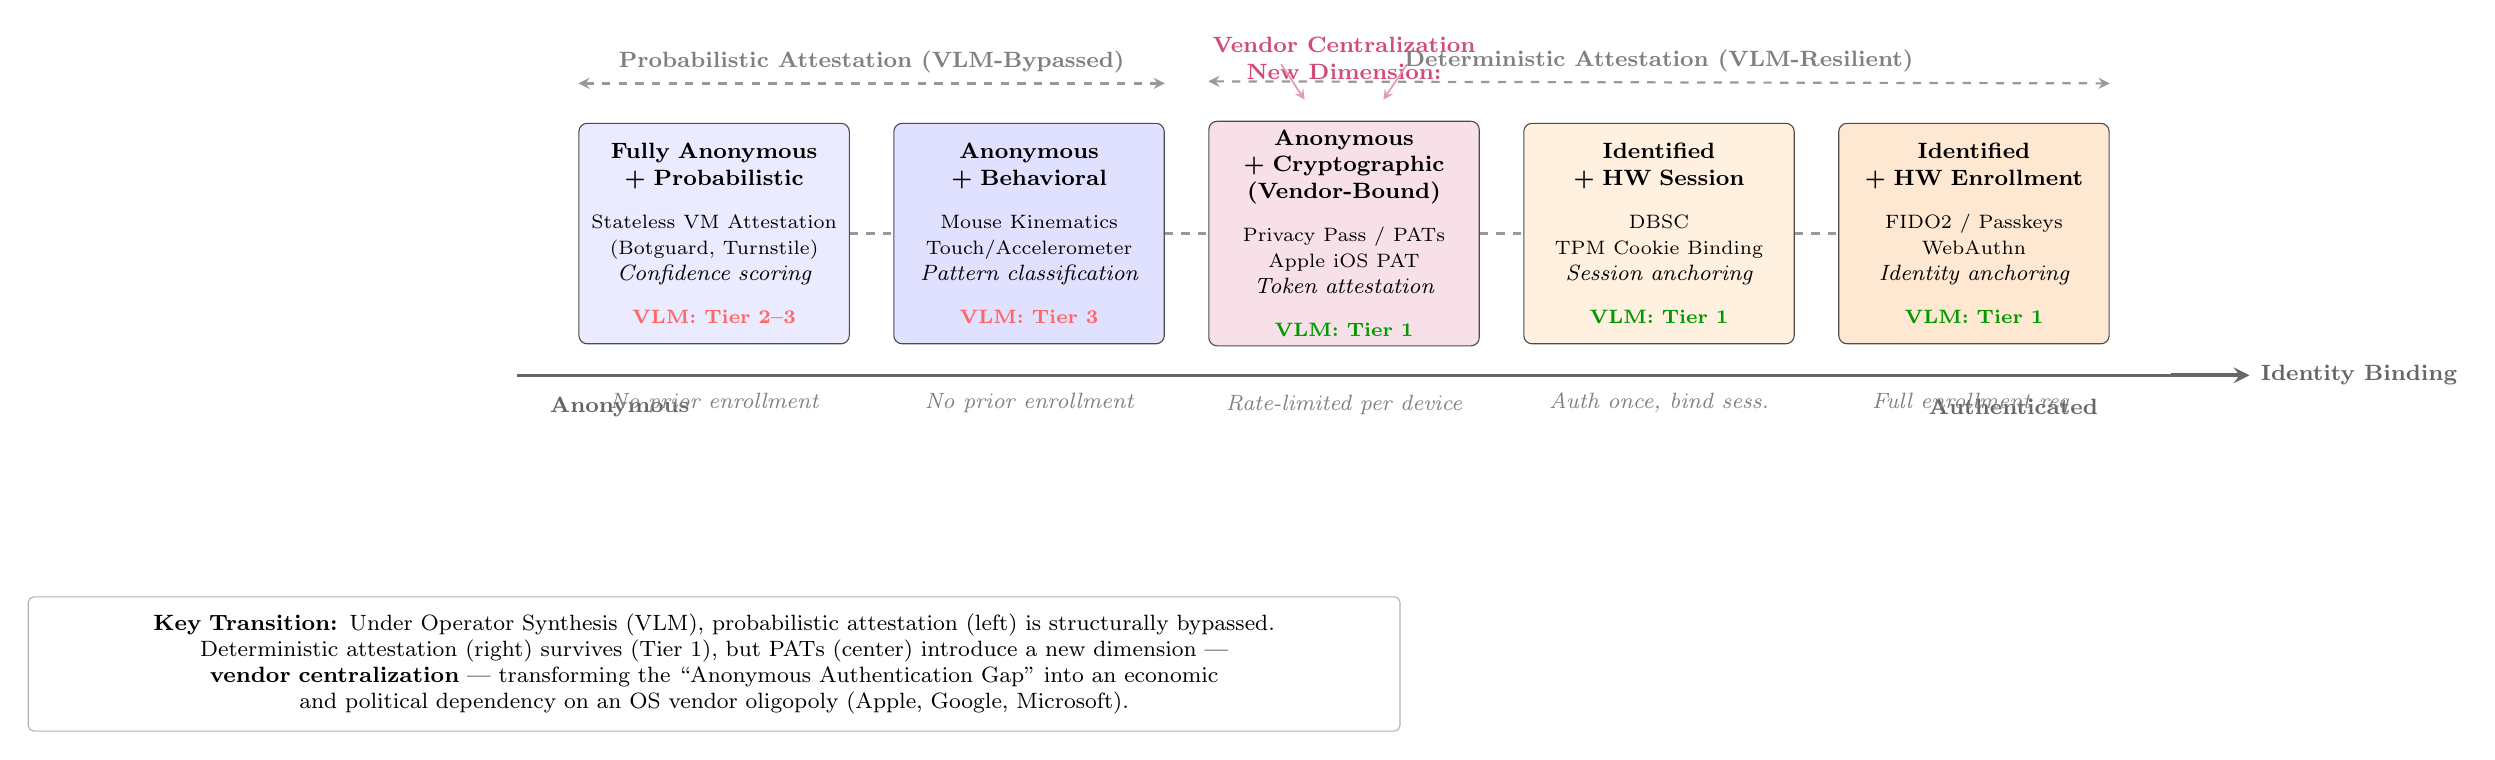
\begin{tikzpicture}[
    scale=1.0,
    spectrum/.style={
        rectangle,
        rounded corners=3pt,
        draw=black!70,
        fill=#1,
        text width=3.2cm,
        align=center,
        minimum height=2.8cm,
        font=\footnotesize
    },
    arrow/.style={
        ->,
        >=stealth,
        line width=1.5pt,
        black!60
    },
    dimarrow/.style={
        <->,
        >=stealth,
        line width=0.8pt,
        black!40,
        dashed
    }
]

% Gradient backgrounds for spectrum boxes
\node[spectrum={blue!8}] (l1) at (0,0) {
    \textbf{Fully Anonymous} \\
    \textbf{+ Probabilistic} \\
    \medskip
    {\scriptsize Stateless VM Attestation} \\
    {\scriptsize (Botguard, Turnstile)} \\
    {\footnotesize\itshape Confidence scoring} \\
    \medskip
    {\scriptsize\bfseries\color{red!60} VLM: Tier 2--3}
};

\node[spectrum={blue!12}] (l2) at (4,0) {
    \textbf{Anonymous} \\
    \textbf{+ Behavioral} \\
    \medskip
    {\scriptsize Mouse Kinematics} \\
    {\scriptsize Touch/Accelerometer} \\
    {\footnotesize\itshape Pattern classification} \\
    \medskip
    {\scriptsize\bfseries\color{red!60} VLM: Tier 3}
};

\node[spectrum={purple!12}] (l3) at (8,0) {
    \textbf{Anonymous} \\
    \textbf{+ Cryptographic} \\
    \textbf{(Vendor-Bound)} \\
    \medskip
    {\scriptsize Privacy Pass / PATs} \\
    {\scriptsize Apple iOS PAT} \\
    {\footnotesize\itshape Token attestation} \\
    \medskip
    {\scriptsize\bfseries\color{green!60!black} VLM: Tier 1}
};

\node[spectrum={orange!12}] (l4) at (12,0) {
    \textbf{Identified} \\
    \textbf{+ HW Session} \\
    \medskip
    {\scriptsize DBSC} \\
    {\scriptsize TPM Cookie Binding} \\
    {\footnotesize\itshape Session anchoring} \\
    \medskip
    {\scriptsize\bfseries\color{green!60!black} VLM: Tier 1}
};

\node[spectrum={orange!18}] (l5) at (16,0) {
    \textbf{Identified} \\
    \textbf{+ HW Enrollment} \\
    \medskip
    {\scriptsize FIDO2 / Passkeys} \\
    {\scriptsize WebAuthn} \\
    {\footnotesize\itshape Identity anchoring} \\
    \medskip
    {\scriptsize\bfseries\color{green!60!black} VLM: Tier 1}
};

% Axis line
\draw[line width=1.2pt, black!60] (-2.5, -1.8) -- (18.5, -1.8);
\draw[arrow] (18.5, -1.8) -- (19.5, -1.8) node[right, font=\footnotesize\bfseries] {Identity Binding};

% Axis labels
\node[font=\footnotesize\bfseries, text=black!60] at (-1.2, -2.2) {Anonymous};
\node[font=\footnotesize\bfseries, text=black!60] at (16.5, -2.2) {Authenticated};

% Spectrum connections
\draw[thick, black!40, dashed] (l1.east) -- (l2.west);
\draw[thick, black!40, dashed] (l2.east) -- (l3.west);
\draw[thick, black!40, dashed] (l3.east) -- (l4.west);
\draw[thick, black!40, dashed] (l4.east) -- (l5.west);

% Top-level categorization brackets
\draw[dimarrow] (l1.north west) ++(0, 0.5) -- node[above, font=\footnotesize\bfseries, text=black!50] {Probabilistic Attestation (\textbf{VLM-Bypassed})} ($(l2.north east) + (0, 0.5)$);
\draw[dimarrow] ($(l3.north west) + (0, 0.5)$) -- node[above, font=\footnotesize\bfseries, text=black!50] {Deterministic Attestation (\textbf{VLM-Resilient})} ($(l5.north east) + (0, 0.5)$);

% Bottom dimension annotations
\node[font=\footnotesize\itshape, text=black!50, below=0.5cm of l1] {No prior enrollment};
\node[font=\footnotesize\itshape, text=black!50, below=0.5cm of l2] {No prior enrollment};
\node[font=\footnotesize\itshape, text=black!50, below=0.5cm of l3] {Rate-limited per device};
\node[font=\footnotesize\itshape, text=black!50, below=0.5cm of l4] {Auth once, bind sess.};
\node[font=\footnotesize\itshape, text=black!50, below=0.5cm of l5] {Full enrollment req.};

% Vendor trust annotation for center column
\node[font=\footnotesize\bfseries, text=purple!70, above=0.4cm of l3] {New Dimension:};
\node[font=\footnotesize\bfseries, text=purple!70] at (8, 2.4) {Vendor Centralization};
\draw[->, >=stealth, purple!40, line width=0.6pt] (7.2, 2.15) -- (7.5, 1.7);
\draw[->, >=stealth, purple!40, line width=0.6pt] (8.8, 2.15) -- (8.5, 1.7);

% Legend box bottom
\node[draw=black!30, fill=white, rounded corners=2pt, font=\footnotesize, text width=17cm, align=center, below=2.2cm of l1.south, yshift=-1.0cm, inner sep=6pt] (legend) {
    \textbf{Key Transition:} Under Operator Synthesis (VLM), probabilistic attestation (left) is structurally bypassed. \\
    Deterministic attestation (right) survives (Tier 1), but PATs (center) introduce a new dimension — \\
    \textbf{vendor centralization} — transforming the ``Anonymous Authentication Gap'' into an economic \\
    and political dependency on an OS vendor oligopoly (Apple, Google, Microsoft).
};

\end{tikzpicture}
\end{document}
